%----------------------------------------
\begin{frame}
  \frametitle{Part 2}

{\Large\bf \promelaname{}: the modeling language}

\end{frame}

%----------------------------------------
\begin{frame}
  \frametitle{\promelaname{} in one slide} \small

{\em Process Meta Language}. C-like syntax, but it is a {\bf modeling} language,
not a programming language.

\vspace{0.3cm}

\begin{itemize}
\item {\bf Processes} (\ipromela{proctype}) --- the units of concurrency.
\item {\bf Channels} (\ipromela{chan}) --- synchronous or buffered message passing.
\item {\bf Global and local variables} --- finite types only (\ipromela{bit}, \ipromela{byte}, \ipromela{short}, \ipromela{int}, \ipromela{mtype}).
\item {\bf Guarded commands} --- \ipromela{if}/\ipromela{fi} and \ipromela{do}/\ipromela{od}, with nondeterministic choice.
\item {\bf Blocking semantics} --- a statement executes only when it is {\em executable}.
\end{itemize}

\pause
\vspace{0.3cm}

\begin{block}{Important idea}\small
In \promelaname{} a {\bf boolean expression is a statement}. It blocks until it is
true. So \ipromela{(x > 0)} on its own line means ``wait until \ipromela{x > 0}''.
\end{block}

\end{frame}

%----------------------------------------
\begin{frame}[fragile]
  \frametitle{Processes} \small

\begin{lstlisting}[language=promela]
byte powered = 0;              /* global, shared */

proctype Instrument(byte id) {
  byte local = 0;              /* local to each instance */
  local = powered;
  powered = local + 1;
  printf("instrument %d on\n", id)
}

init {
  run Instrument(1);           /* spawn */
  run Instrument(2)
}
\end{lstlisting}

\pause

Statements of different processes interleave arbitrarily --- {\bf that is the
point}.

\end{frame}

%----------------------------------------
\begin{frame}[fragile]
  \frametitle{Guarded commands: \tool{if}} \small

\begin{lstlisting}[language=promela]
/* the environment: temperature does what it likes */
if
:: (t < 120) -> t = t + 10        /* it rises           */
:: (t >   0) -> t = t - 10        /* it falls           */
:: true      -> sensor = FAILED   /* or the sensor dies */
fi
\end{lstlisting}

\pause
\vspace{0.2cm}

\begin{block}{Semantics}\small
\begin{itemize}
\item Every guard is evaluated. {\bf All} true guards are candidates.
\item One of them is chosen {\bf nondeterministically}. For $0 < t < 120$ all
      three hold, and \spin{} explores {\bf all three} branches.
\item Guard order is irrelevant --- this is not C's \tool{else if}.
\item If no guard is true and there is no \ipromela{else}, the \ipromela{if} {\bf blocks}.
\end{itemize}
\end{block}

\pause
\vspace{0.2cm}

{\bf Nondeterminism is a modeling tool}, not a bug. No branch here is the
``right'' one: whatever you prove holds for {\em every} environment behavior,
including the sensor failing at the worst possible moment.

\end{frame}

%----------------------------------------
\begin{frame}[fragile]
  \frametitle{Guarded commands: \tool{do}} \small

\begin{lstlisting}[language=promela]
/* the same environment, now running forever */
do
:: (t < 120) -> t = t + 10
:: (t >   0) -> t = t - 10
:: true      -> sensor = FAILED; break
od
\end{lstlisting}

\vspace{0.2cm}

Same choice rule, repeated forever until \ipromela{break} or \ipromela{goto}.
The temperature now wanders over every reachable value, and the sensor may fail
at {\bf any} point along the way.

\end{frame}

%----------------------------------------
\begin{frame}[fragile]
  \frametitle{Channels} \small

\begin{lstlisting}[language=promela]
mtype = { HEAT, COOL, ACK };          /* symbolic constants */

chan cmd  = [0] of { mtype, byte };   /* rendezvous  */
chan tlm  = [8] of { mtype, byte };   /* buffered, capacity 8 */

cmd ! HEAT, 42;      /* send    */

mtype msg; byte value;
tlm ? msg, value;    /* receive */
\end{lstlisting}

\pause
\vspace{0.2cm}

\begin{itemize}
\item Capacity \ipromela{[0]} $\Rightarrow$ {\bf synchronous} handshake: sender and
      receiver move together.
\item Capacity $>0$ $\Rightarrow$ {\bf asynchronous} FIFO; send blocks when full,
      receive blocks when empty.
\item \ipromela{len(ch)}, \ipromela{empty(ch)}, \ipromela{full(ch)}, \ipromela{nempty(ch)}, \ipromela{nfull(ch)}.
\item \ipromela{ch ? eval(x)} matches only a message equal to the current value of \ipromela{x};
      \ipromela{ch ? [msg, value]} tests receivability without consuming.
\end{itemize}

\end{frame}

%----------------------------------------
\begin{frame}[fragile]
  \frametitle{Modeling an unreliable channel} \small

\begin{lstlisting}[language=promela]
do
:: link ? msg ->
     if
     :: out ! msg              /* delivered    */
     :: skip                   /* silently lost */
     :: out ! msg; out ! msg   /* duplicated   */
     fi
od
\end{lstlisting}

\vspace{0.25cm}

{\centering
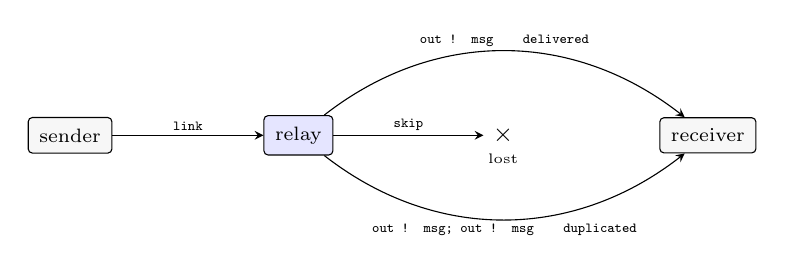
\begin{tikzpicture}[
  font=\scriptsize, >=stealth,
  b/.style={draw, rounded corners=1.5pt, align=center, inner sep=4pt,
            fill=black!3},
  lab/.style={font=\tiny, inner sep=1.5pt}
]
  \node[b] (s) at (0,0)                  {sender};
  \node[b, fill=blue!10] (r) at (2.9,0)  {relay};
  \node[b] (d) at (8.1,0)                {receiver};

  \draw[->] (s) -- node[lab, above] {\tt link} (r);

  \draw[->] (r) to[out=38,in=142]
        node[lab, above] {\tt out ! msg \ \ \ delivered} (d);
  \node[font=\small] (x) at (5.5,0) {$\times$};
  \draw[->] (r) -- node[lab, above] {\tt skip} (x);
  \node[lab] at (5.5,-0.3) {lost};
  \draw[->] (r) to[out=-38,in=-142]
        node[lab, below] {\tt out ! msg; out ! msg \ \ \ duplicated} (d);
\end{tikzpicture}\par}

\pause
\vspace{0.25cm}

Three lines of nondeterminism replace an entire fault-injection harness.
Every property you then prove holds under loss and duplication.

\end{frame}

%----------------------------------------
\begin{frame}[fragile]
  \frametitle{Atomicity} \small

By default, {\bf every statement is a possible preemption point}.
Two ways to say otherwise:

\vspace{0.3cm}

\begin{lstlisting}[language=promela]
atomic { t = x; x = t + 1 }   /* atomicity lost if it blocks */

d_step { t = x; x = t + 1 }   /* one step, may never block  */
\end{lstlisting}

\pause
\vspace{0.3cm}

\begin{block}{Why you care}\small
\begin{itemize}
\item \ipromela{atomic} and \ipromela{d_step} are how you model a critical section,
      a disabled-interrupt region, or a hardware-atomic instruction.
\item They are also the main lever for {\bf reducing the state space}: fewer
      interleaving points means exponentially fewer states.
\item {\bf Danger:} over-using them hides the very bugs you are looking for.
\end{itemize}
\end{block}

\end{frame}

